\documentclass{beamer} % bemutatóhoz: \documentclass{beamer}
\usepackage{t1enc}
\usepackage{ragged2e}
\let\raggedright=\RaggedRight
\usepackage[utf8]{inputenc}
\usepackage{amsmath}
\usepackage{amsfonts}
\usepackage{amssymb}
\usepackage{amsthm}
\usepackage{mathrsfs}
\usepackage{mathptm}
\usepackage{physics}
\usepackage{times}
\newtheorem{lem}{Lemma}[section]
\newtheorem{theo}[lem]{Theorem}
\newtheorem{defi}[lem]{Definition}
\newtheorem{megall}[lem]{Megállapodás}
\newtheorem{allitas}[lem]{Proposition}
\newtheorem{atfog}[lem]{Átfogalmazás}
\DeclareMathOperator{\dom}{dom}
\DeclareMathOperator{\ess}{ess}
\DeclareMathOperator*{\ch}{ch}
\usetheme{Madrid}
\setbeamertemplate{footline}{}
\setbeamertemplate{navigation symbols}{}
\title{On the list coloring of $1$-band buffering graphs}
\subtitle{Introduction to the theory}
\author{Benjámin Martin Seregi}
\institute{
      %\includegraphics[scale=0.2]{elte_cimer_szines}%
      \\[\medskipamount]
      KTH Royal Institute of Technology \\ II2202, Fall 2017, Period 1-2
}
%\titlegraphic{\includegraphics[]{elte_cimer_szines}}
\date{2017}
\begin{document}
\frame{\titlepage}

\begin{frame}
\frametitle{$1$-band buffering cellular graphs and their list-coloring coloring}
\justifying
\begin{itemize}
\item A graph $G$ is cellular if it is constructed from a hexagonal cellular topology and
\pause \item we say that it is $1$-band buffering if the interference extends up to $1$ cell.
\end{itemize}
\pause \begin{defi}[$k$-choosability and $k$-list coloring]
Let $G$ be a graph and $L(v)$ a set of colors for all $v \in V(G)$ such that $|L(v)|=k$. We say that $G$ is $k$\textit{-choosable} if $G$ is colorable such that the color of $v$ is in $L(v)$ for all $v \in V(G)$, such colorings called $k$\textit{-list coloring} of $G$.
\end{defi}
\end{frame}

\begin{frame}
\frametitle{Why is it important to study this?}
\justifying
\begin{itemize}
\item A $k$-list coloring of a cellular graph corresponds to an interference-free channel allocation where $L(v)$ is the list of free channels for the access point $v$.
\pause \item Finding the optimal channel allocation is of great interest: with interference-free allocations it is possible to achieve higher throughput.
\pause \item Channel allocation problem is $\mathrm{NP}$-complete in general.
\end{itemize}
\begin{figure}
\caption{3-coloring of a cellular graph, $L(v):=\lbrace \text{PURPLE,YELLOW,BLUE} \rbrace.$}
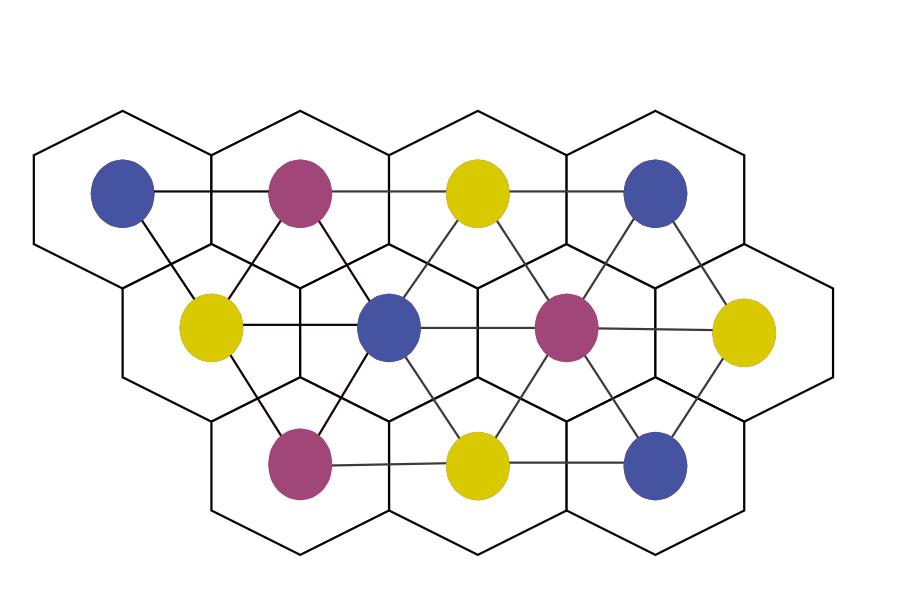
\includegraphics[scale=0.15]{3_coloring_cellular.png}
\end{figure}
\end{frame}

\begin{frame}
\frametitle{Research questions}
\justifying
\begin{itemize}
\item What is the smallest $k > 0$ such that a cellular graph is $k$-choosable (i.e. what is the choice number of cellular graphs)?
\pause \item Can we construct a $k$-list coloring in polynomial time (where $k$ is close or equal to the choice number)?
\end{itemize}
\end{frame}

\begin{frame}
\frametitle{Answers}
\justifying
\begin{itemize}
\item If $G$ is cellular then $\ch(G) \leqslant 4$ (see Research plan, Appendix II)
\pause \item There exists a polynomial time algorithm that constructs a $4$-list coloring for such graphs.
\end{itemize}
\end{frame}


\begin{frame}
\frametitle{The algorithm}
\justifying
The algorithm is based on Galvin's theorem (IV. Hypothesis):
\begin{theo}[Galvin, 1995] Let $G$ be a graph and $\lbrace L(v) : v \in V(G) \rbrace$ given color sets. If $G$ has an orientation $D$ such that $d^+(v) < |L(v)|$ for all $v \in V(D)$ and every induced subgraph of $D$ has a kernel, then $G$ can be colored from the given color sets.
\end{theo}
\pause Outline of the proof of our algorithm:
\begin{itemize}
\item If $G$ is cellular then it has a $3$-bounded acyclic orientation that can be computed in polynomial time (Research Plan, Appendix I).
\pause \item Acyclic graphs are kernel-perfect and a kernel can be constructed in polynomial time (see my branch: final-report-theory, Research Plan VII. Research Methodology).
\pause \item Apply Galvin's theorem.
\end{itemize}
\end{frame}

\end{document}